\chapter{Project Development}
	
In each of the previous chapters I have explored different aspects of the fields of home automation and voice assistance from a 
theoretical point of view, from their definition to smaller details, including additional explanations about a specific home automation 
system, openHAB.

At this time, I think I have provided enough background to begin my case study: the building of a home automation controller. As I 
mentioned in the openHAB chapter, I will base my project on this system and build on it, as it accomplishes very well the main
requirements that I determined for this project.

In this chapter, I will detail the process that I have followed in order to develop this project, from its specification to the final result.

\section{Product Specification}
The first task to do is to define the product. What should a home automation system do? What do users expect it to do? How? All 
the answers to these questions can be clarified by following some processes that, although they do not completely answer them (we 
can see many failed projects from time to time), they provide a very clear and detailed specification from the beginning.

\subsection{Personas}
Creating personas is a common process applied to the product design and development process in order to help in making a user-centered
design, and it is applicable in this project in order to have a better idea of what would users expect from the final product.

A persona is a representation of a user, typically based off user research and incorporating user goals, needs, and interests.

In this project, I am going to use proto-personas, which are based on secondary research and the guess of who they should be designed 
for, as currently we do not have means and time for making true research-based personas (and it is not the main objective in this project).

After thinking about the main uses of this system and the people that would be interested on it, I have extracted these three personas, 
representing its main uses, although not the only ones. I have built them with the online platform Xtensio, and the figures
\ref{fig:persona-oswald-douglas}, \ref{fig:persona-anna-lahtinen} and \ref{fig:persona-rosario-vera} represent them. I tried to extract 
a varied range of backgrounds, current situations, desires and worries. 

Oswald Douglas (figure \ref{fig:persona-oswald-douglas}) is a freelance technology blogger from Dallas, USA, that is very interested 
in the areas of home automation and Internet of Things. He is looking to automate his own home and write about his experience in 
his blog. He already has experience with technology, and this next step will not be too difficult for him. His interests are clear: 
to try cutting-edge technology in his own home and make the most of home automation.

Anna Lahtinen (figure \ref{fig:persona-anna-lahtinen}) is a 16 year-old high school student from Lappeenranta, Finland. She is up 
to date on technology but she is not passionate about it. However, she heard about home automation and thinks that she could enjoy 
a better media experience with it. In addition, she thinks that adding smart color light bulbs to her bedroom would make it look more 
beautiful. However, she feels that there is a lack of general information about devices and the set up and configuration of a home 
automation system. She thinks that the price of it is too high as well.

Rosario Vera (figure \ref{fig:persona-rosario-vera}) is an administrative from Vitoria-Gasteiz, Spain. She is 37 years old, is married and 
has two young children. She is not very familiar with technology, but she has heard about home automation in the news and thinks 
that it could fit her needs. Rosario and her husband work outside home, and sometimes their children need to be alone at home. Home 
automation would provide more security to the home and would allow them to have more spare time. Voice assistance would be helpful 
for their children when they are alone, as it is a very easy and natural way to interact with technology. However, she is concerned about 
their privacy regarding these systems and she thinks that companies should give more accessible explanations about it. In addition, 
she finds these systems difficult to use.

\begin{sidewaysfigure}
	\centering
	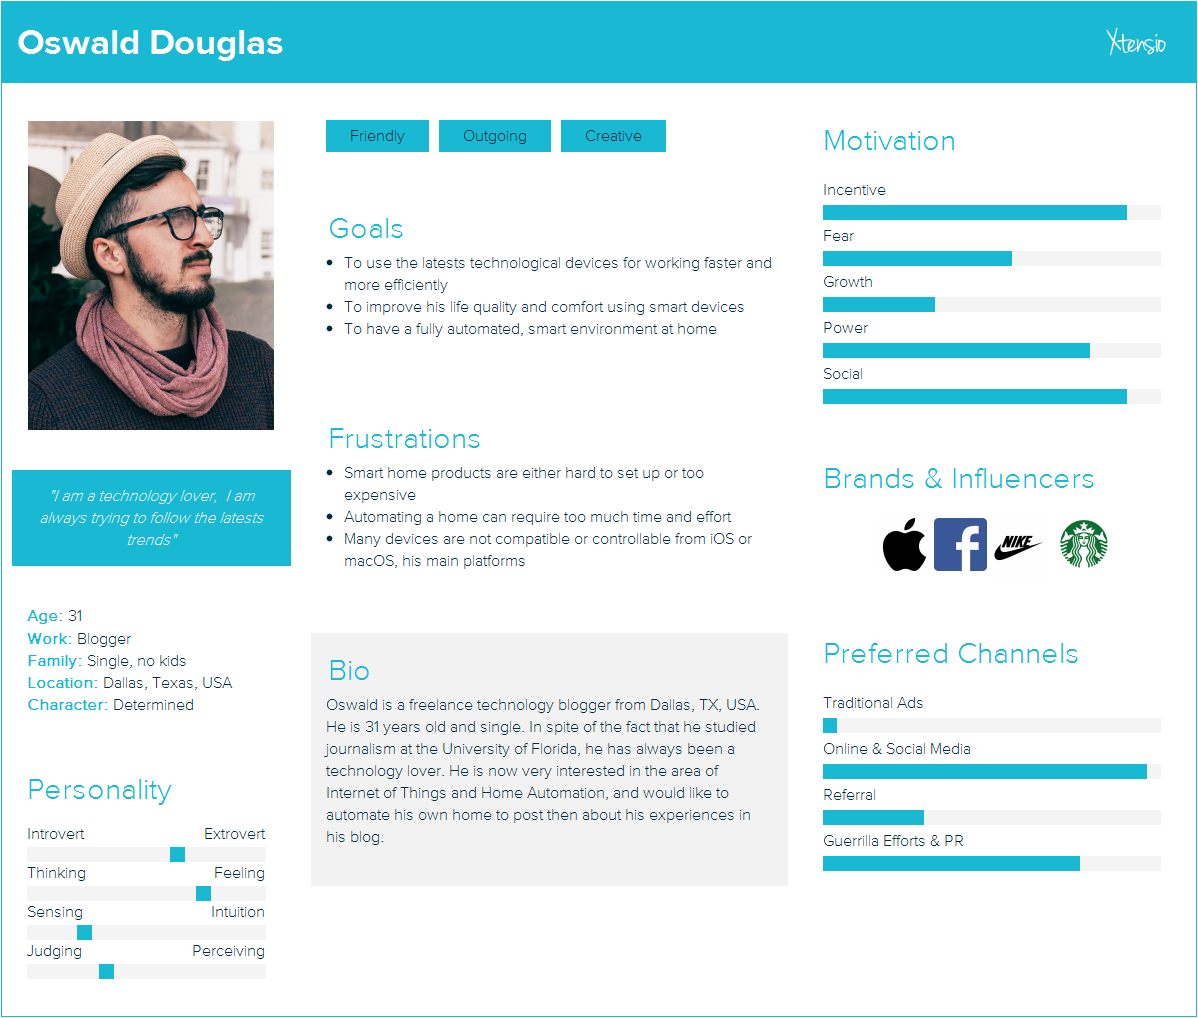
\includegraphics[width=0.65\textwidth]{images/Chapter_06/persona-oswald-douglas.png}
	\caption{Persona: Oswald Douglas}
	\label{fig:persona-oswald-douglas}
\end{sidewaysfigure}

\begin{sidewaysfigure}
	\centering
	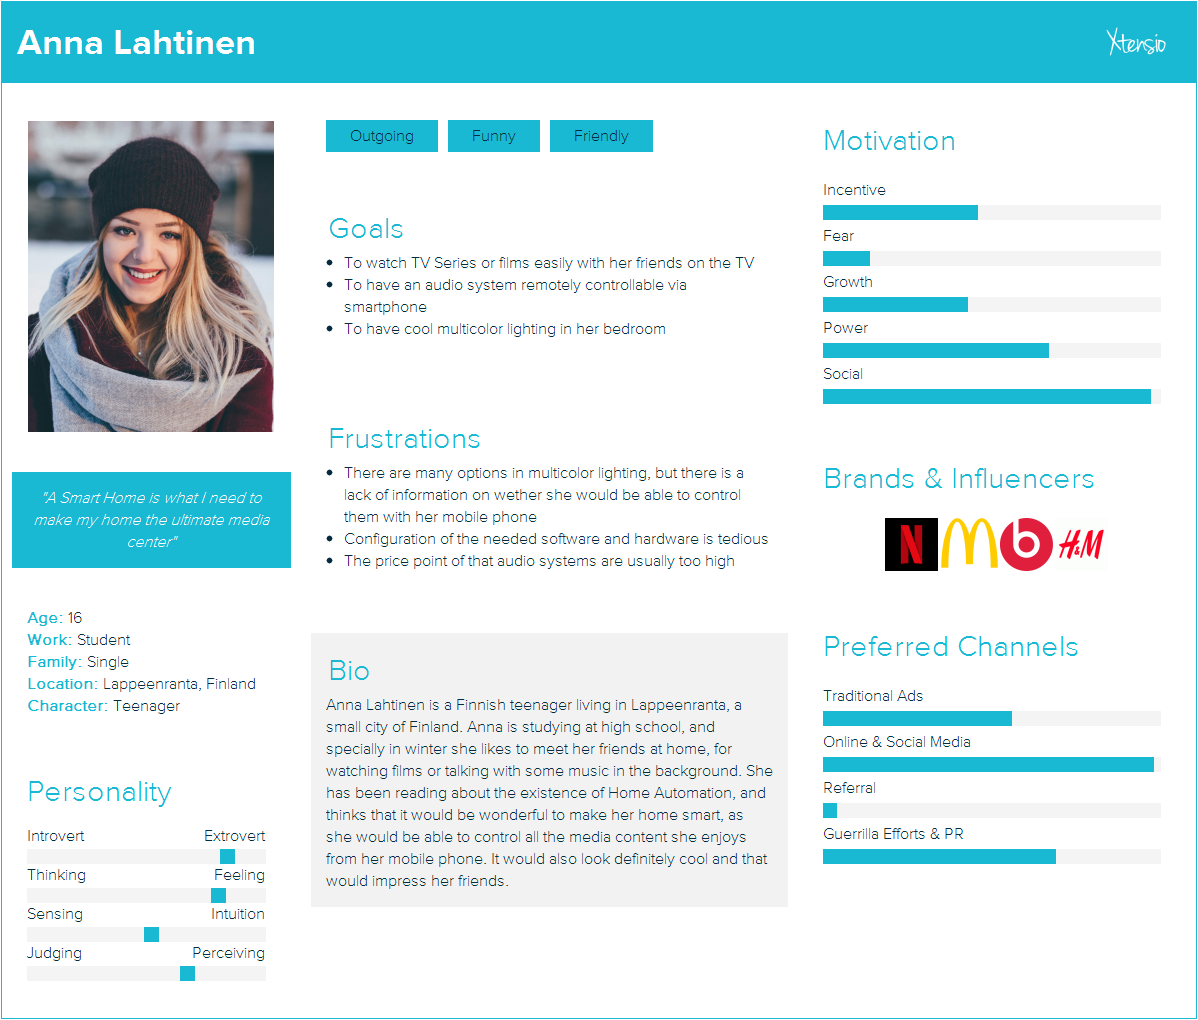
\includegraphics[width=0.65\textwidth]{images/Chapter_06/persona-anna-lahtinen.png}
	\caption{Persona: Anna Lahtinen}
	\label{fig:persona-anna-lahtinen}
\end{sidewaysfigure}

\begin{sidewaysfigure}
	\centering
	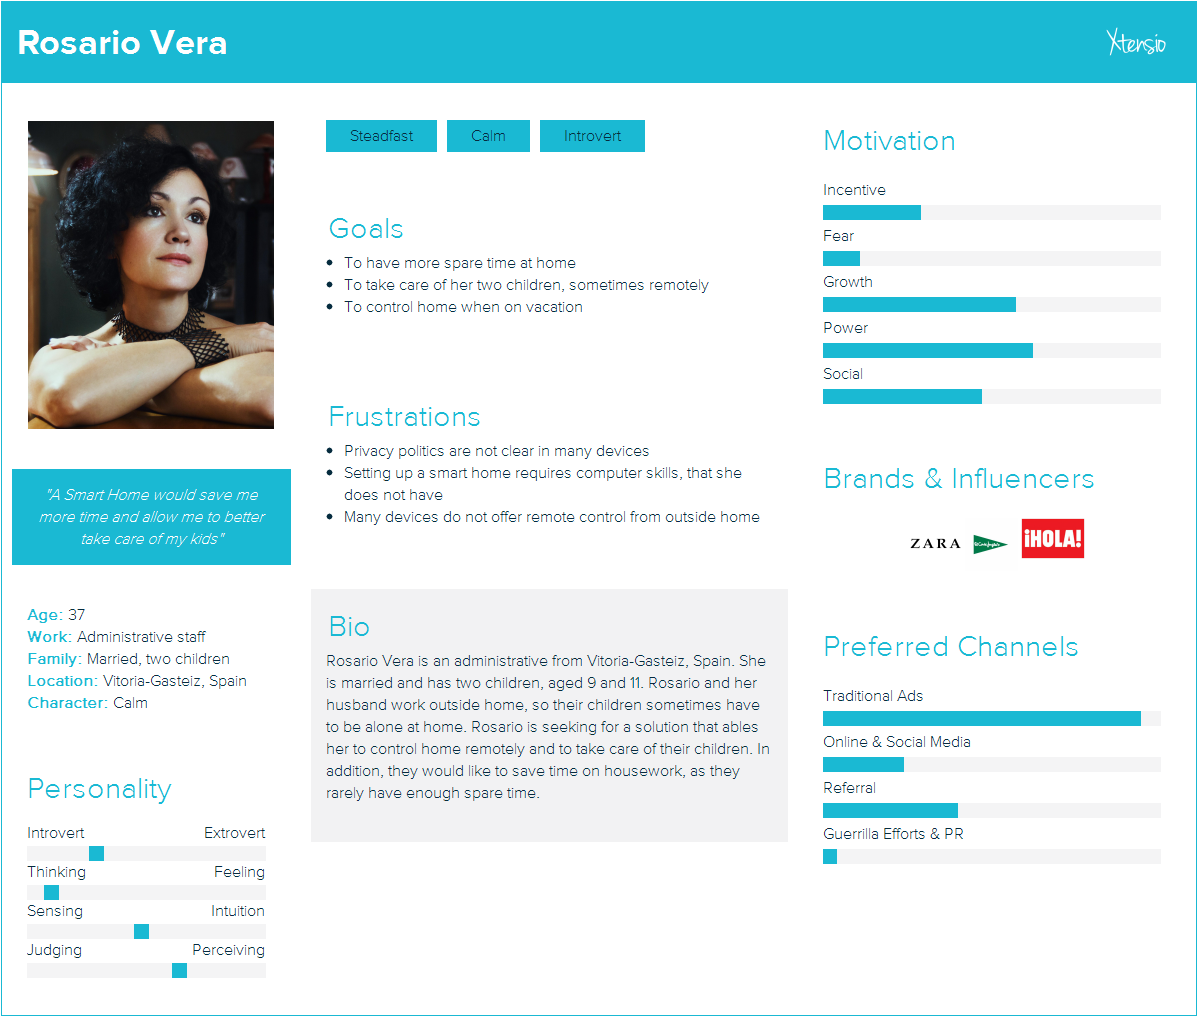
\includegraphics[width=0.65\textwidth]{images/Chapter_06/persona-rosario-vera.png}
	\caption{Persona: Rosario Vera}
	\label{fig:persona-rosario-vera}
\end{sidewaysfigure}

\subsection{Software Requirements Specification}
With the Software Requirements Specification (SRS), I try to describe the project to develop from a functional point of view, that is,
to determine the capabilities that the software system will have.

The domotic controller will be able to control all modern devices in our home, regardless of their maker and the technology they use.
It will provide an easy to use user interface and the ability to easily install, modify or remove the devices. It will also include natural
human-computer interaction through the voice. A more detailed specification of the requirements can be found in the subsections
below.

\subsubsection{Functional Requirements}
Functional requirements are a description of the facility or feature required. They deal with what the system should do or provide 
for users.\cite{sqaFunctionalNonFunctional}

\begin{itemize}
	\item \textbf{FR1}: The system will be able to retrieve automatically the status of the different properties of the elements.
	\item \textbf{FR2}: The system will be able to retrieve automatically data from its different data providers.
	\item \textbf{FR3}: The system will not need any operation to launch openHAB after it is powered on.
	\item \textbf{FR4}: The system will be able to turn itself off safely.
	\item \textbf{FR5}: The system will automatically detect new smart devices connected to the local network.
	\item \textbf{FR6}: The system will be able to detect the possible operations with each connected smart device. 
	\item \textbf{FR7}: The system will be able to operate with the connected devices according to the detected possible operations.
	\item \textbf{FR8}: The system will be able to tell the user in an understandable manner the current connection status for each
	device.
	\item \textbf{FR9}: The system will provide different user interfaces, so users can choose one between them, according to
	their needs.
	\item \textbf{FR10}: The user will be able to change the configuration of the system from a graphical user interface.
	\item \textbf{FR11}: The system will be manually configurable and modifiable using configuration files.
	\item \textbf{FR12}: The system will automatically include and configure new devices found in the network, after the user decides
	to add them.
	\item \textbf{FR13}: The user will be able to configure the name, display icon, IP and all possible aspects of the item directly from
	the user interface.
	\item \textbf{FR14}: The system will allow the user to make groups of items.
	\item \textbf{FR15}: The system will allow the user to add groups of items to other groups of items.
	\item \textbf{FR16}: The system will be modular and include a package system. Each package supports a set of devices.
	\item \textbf{FR17}: The package system will be accessible from the graphical user interface.
	\item \textbf{FR18}: The installation of packages will be done automatically after the user clicks on the install button.
	\item \textbf{FR19}: The removal of packages will be done automatically after the user clicks on the remove button.
	\item \textbf{FR20}: The system will maintain an updated and classified list of packages according to an external repository.
	\item \textbf{FR21}: The system will be manageable from external sources.
	\item \textbf{FR22}: The system will be accessible from external devices and from the Internet.
	\item \textbf{FR23}: The system will allow to have automation rules defined by the user.
	\item \textbf{FR24}: The voice assistant will allow to perform the main operations of each device in the system.
	\item \textbf{FR25}: The voice assistant will be able to answer in different languages.
	\item \textbf{FR26}: The voice assistant will be able to do power management tasks in the system, such as powering the system
	off or restarting the system.
	\item \textbf{FR27}: The voice assistant will be operable through mechanical methods or by voice.
	\item \textbf{FR28}: The users will be able to edit and adapt the functionalities of the voice assistant according to their needs.
	\item \textbf{FR29}: The voice assistant will provide spoken feedback if there has been an error performing the given command.
	\item \textbf{FR30}: The voice assistant will be able to print debug information in the command line if it is required.
\end{itemize}

\subsubsection{Non-Functional Requirements}
Non-functional requirements detail constraints, targets or control mechanisms for the new system. They describe how, how well or
to what standard a function should be provided.\cite{sqaFunctionalNonFunctional}

\begin{itemize}
	\item \textbf{NFR1}: The system, along with the voice assistant, will be installable in the Raspberry Pi.
	\item \textbf{NFR2}: The system and the voice assistant will provide a satisfactory response rate.
	\item \textbf{NFR3}: The user interfaces of the home automation system will be adaptable to the size and resolution of the
	user's screen.
	\item \textbf{NFR4}: The user interfaces will be made according to modern standards, like Material Design.
	\item \textbf{NFR5}: The home automation system will run in a local server, created in the machine which executes it.
	\item \textbf{NFR6}: In order to allow external connections, the home automation system will provide a REST API.
	\item \textbf{NFR7}: The system will provide secure access options.
	\item \textbf{NFR8}: The system must be available the 99\% of the time.
	\item \textbf{NFR9}: The system must be scalable.
	\item \textbf{NFR10}: The system must be recoverable in less than 45 minutes.
	\item \textbf{NFR11}: The cost of the system must me minimal.
	\item \textbf{NFR12}: The system must be interoperable with multiple devices.
	\item \textbf{NFR13}: The voice assistant will recognize English.
	\item \textbf{NFR14}: The voice assistant will be fast in its response. Therefore, its procedure for deciding a response will 
	be optimal.
	\item \textbf{NFR15}: The voice assistant will operate with the home automation system via REST, so it can be installed in a
	different computer than the one with the home assistant.
\end{itemize}

\subsection{Use Cases}
The next step after the specification of requirements is to specify the use cases of the system.

Use case diagrams are usually referred to as behavior diagrams used to describe a set of actions (use cases) that some system or 
systems (subject) should or can perform in collaboration with one or more external users of the system (actors).\cite{umlUseCaseDiagrams}

%TODO
%Hacer los diagramas de casos de uso tal y como indiqué en UC-device-and-service-control.xml
%Dividir los requisitos de modo que queden subsistemas funcionales diferenciados

\subsection{Functional Subsystems}
%TODO
%Especificar aquí los subsistemas funcionales

\subsection{Implementation Possibilities}
After exploring what users would expect from a system like this, it is worth thinking about how it should be implemented. Together 
with my director, I proposed different options to meet the previous requirements.

\subsubsection{Web Platform}
A well designed web platform is a great idea nowadays. If this platform is hosted in a local server, it means that it can be accessed
from any device connected to the network. With the correct configuration, it could be even reachable from anywhere in the world.
It is easy to implement and maintain, and users with basic web development knowledge would be able to easily modify it. In addition,
the same web platform can be adaptable to any device and resolution, thanks to responsive designs. It would also work if we attach
a tactile screen to the Raspberry Pi.

OpenHAB mounts a web platform in a local server by default, and provides several adaptable user interfaces, so this solution would
not require much effort, and it offers many possibilities.

\subsubsection{Desktop Application}
Another solution, focused on the Raspberry Pi desktop (where we mainly want to implement the system), is developing a desktop 
application with an adapted user interface for tactile screens. The advantage of a desktop application is that it usually requires 
less resources and it is faster, but it is a specific solution for the Raspberry Pi, so it would only work there. We would need a 
different application if we wanted it to run on mobile phones or tablets.

We would need to make it from scratch, as openHAB does not provide any desktop application.

\subsubsection{Mobile Application}
Mobile phones and \textit{tablets} are common devices that are widely used to manage smart homes. Some setups have a tablet located 
somewhere in the home, which is only used for managing the domotic devices. An application is faster and more accessible than a web
platform, and users are more used to them, so it would be convenient in some cases.

However, making the system only accessible from a mobile or tablet application would reduce the utility of the Raspberry Pi, and 
would at least require two devices (one for the local server and another one for accessing it). Although it is a good complement to the
system, it is not convenient to base it only on a mobile application. However, it is applicable in a hybrid solution.

\subsubsection{Hybrid Solution}
A hybrid solution consists of applying two or more solutions together of those specified above. For example, providing a web platform 
and an optional mobile application to easily manage the system from a mobile device.

OpenHAB provides a web platform, as explained above, and a mobile application for iOS and Android than connects to the web platform.

\subsubsection{Comparison}
The table \ref{table:possible-implementations} compares all the possibilities for the implementation of the system.

\begin{table}[]
	\centering
	\resizebox{\textwidth}{!}{%
		\begin{tabular}{|l|c|c|c|c|}
			\hline
			\multicolumn{1}{|c|}{\textbf{Feature}}                                  & \textbf{\begin{tabular}[c]{@{}c@{}}Web\\ platform\end{tabular}} & \textbf{\begin{tabular}[c]{@{}c@{}}Desktop \\ application\end{tabular}} & \textbf{\begin{tabular}[c]{@{}c@{}}Mobile\\ application\end{tabular}} & \textbf{\begin{tabular}[c]{@{}c@{}}Hybrid\\ Solution\end{tabular}} \\ \hline
			\begin{tabular}[c]{@{}l@{}}Support for \\ multiple devices\end{tabular} & Yes                                                             & Only PCs                                                                & \begin{tabular}[c]{@{}c@{}}Only mobile\\ phones/tablets\end{tabular}  & Yes                                                                \\ \hline
			\begin{tabular}[c]{@{}l@{}}Allows access\\ from Internet\end{tabular}   & Yes                                                             & No                                                                      & No                                                                    & Yes                                                                \\ \hline
			\begin{tabular}[c]{@{}l@{}}Control from\\ Raspberry Pi\end{tabular}     & Yes                                                             & Yes                                                                     & No                                                                    & Yes                                                                \\ \hline
			\begin{tabular}[c]{@{}l@{}}Easy \\ implementation\end{tabular}          & Yes                                                             & No                                                                      & No                                                                    & Yes                                                                \\ \hline
			\begin{tabular}[c]{@{}l@{}}Maximum\\ performance\end{tabular}           & No                                                              & Yes                                                                     & Yes                                                                   & Partially                                                          \\ \hline
		\end{tabular}%
	}
	\caption{Comparison between possible implementations}
	\label{table:possible-implementations}
\end{table}

As we can see, the hybrid solution, which is a web platform and mobile application, meets all the features in the best way, and 
offers easy and fast implementation. At this point, I have not considered the implementation of the voice assistant, which I will 
talk about in following sections.

\bigskip
\section{System Analysis}
%TODO
%Introducir la sección

\subsection{Conceptual Model}
%TODO
%Especificar el modelo conceptual

\bigskip
\section{System Design}
%TODO
%Introducir la seccion

\subsection{Architecture}
%TODO
%Especificar la arquitectura del sistema, se puede hacer una explicacion rapida de los subsistemas que lo componen

\subsection{Conceptual Class Diagram}
%TODO
%Introducir y especificar el DCC

\bigskip
\section{Implementation}
In this section, I will explain the process that I have followed to implement the home automation controller, along with the voice
assistant.

\begin{figure}
	\centering
	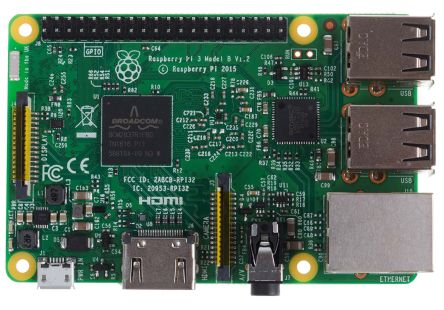
\includegraphics[width=0.8\textwidth]{images/Chapter_06/raspberry-pi-3b.jpg}
	\caption{Raspberry Pi 3}
	\label{fig:raspberry-pi-3b}
\end{figure}

As I have mentioned before, the main objective is to install the system in a Raspberry Pi, which is an affordable and small computer,
with enough power and connectivity options to install a home automation system on it, and even a voice assistant. The possibilities 
of this device are endless: it can work with or without display, and has a special connector to which the user can connect screens, 
microphones, speakers and many other accessories. It also has USB ports on its high-end models, and accepts all the USB 
accessories that a normal computer would accept.

The first approach to this system was to install Raspbian, a Linux distribution provided by openHAB, over a Raspberry Pi 3 Model B+ 
(figure \ref{fig:raspberry-pi-3b}). Raspbian has openHAB preinstalled and configured, so it is ready to use. The first idea was to 
have a computer with openHAB and then a voice assistant in other machine. I installed the distribution on this mini PC, but after 
reviewing the possible voice assistants, I found that it was not the best way to implement it. 

I found the Google AIY Voice Kit, which is a kit provided by Google to makers that want to play around with voice recognition.
They provide a package with some accessories for the Raspberry Pi and a cardboard box that is meant to contain the board and the
accessories. Then, I reconsidered the architecture. It would be also possible to install openHAB in the same machine as the virtual
assistant. This way, we would need just one machine for all. It would be a voice assistant, but with a local server, accessible from
all the devices connected to the local network. It would be possible to attach a screen to it as well, so the user can manage the
smart home graphically from the same device.

I thought this would be the best solution, and it would still meet all the requirements specified previously. So, I began working on it.

\subsection{Introduction to Google AIY Voice Kit}
The AIY Voice Kit is a do-it-yourself project created by Google that demonstrates how easy and inexpensive can be to create a natural 
voice recognizer that works with Google Assistant, at a price of only EUR 30 in Europe. The project, aimed for makers, also lets the 
user add their own questions, which is the most powerful part for our purpose. 

The idea is to adapt the device in order to fetch the voice commands that the microphone captures and manage them in OpenHAB, 
making the system act following user’s instructions.

First of all, I will explain the making and setting up process.





